\setchapterpreamble[o]{%
  \dictum[Intel Corporation]{\textit{``Virtualization is a paradigm shift; it
    changes how you think about your resources.''}}}

\chapter{Introduction}
\label{cha:intro}

Virtual machine (VM) technology is a major development in computer systems
design    \cite{buzen73}.     It    has   extended    the    multi-access,
multi-programming  and multi-processing  systems  to be  multi-environment
systems  as well by  providing efficient  ``copies'' of  complete computer
systems \cite{goldberg73}.

Todays  personal   computer  systems   are  powerful  enough   to  provide
virtualization  technology, which  has long  time been  reserved  for high
performance  mainframe  systems. The  paper  \emph{Analysis  of the  Intel
  Pentium's    Ability    to   Support    a    Secure   Virtual    Machine
  Monitor}\cite{robin00analysis}  discusses the  problems  of how  virtual
machines can be efficiently supported by the IA32 architecture.

In  the last few  years, the  remote execution  of applications  gained on
importance, because powerful server systems need not be maintained locally
but  could be  deployed elsewhere.  Grid  middle-wares such  as Globus  or
Unicore  are examples  for environments,  in  which users  can send  their
computation to  some computer  connected to the  grid and get  the results
back.

This work  is about  the execution of  arbitrary applications on  a remote
system exploiting  virtual machines. In  grid environments it is  always a
problem of  how a  user application  can be made  available on  the remote
systems.  It  addresses  the  problem  that  multiple  potentially  broken
applications are  typically executed on remote  hosts side by  side --- if
one  application behaves  ``wrong'' (e.~g.~CPU  cycle  consumption, memory
leakage,  etc.)  it  may involve  other applications  running on  the same
host.

Sharing of computing resources must always consider security, availability
of  the resources and  fairness among  the resource  users.  To  make that
clear,  take  two jobs  from  different users  that  are  scheduled to  be
executed on the  same grid-node with overlapping execution  times. Let one
of the jobs have  a memory leak --- which is not  as uncommon as you might
think --- that task will eventually  eat up all the available memory. This
misbehavior not only  harms the other job, but also  may harm the software
used to connect the host to the grid.

The here  proposed solution is separation using  virtual machines provided
by  the Xen  hypervisor. Each  job  will be  executed in  its own  virtual
machine and  is not  able to harm  either other  jobs running on  the same
physical host, or the physical node itself.

\section{The history of virtualization technologies}
\label{sec:virtualization-history}

The history of virtualization starts  with a paper entitled ``Time sharing
in  large,  fast  computers''  \cite{Strachey59}  written  by  Christopher
Strachey in  1959. His idea bases  on a single-CPU  system which processes
jobs one  after each  other. If  a program blocks  due to  some peripheral
access the  next program in the queue  gets started and will  be run until
the next peripheral  access occurs and so forth.   The system presents the
user with  a \emph{logical CPU} and  a scheduler assigns  this logical CPU
transparently  for   the  user  to   a  physical  CPU.   His   concept  of
``time-sharing''  is now  known  as \emph{\gls{glo:multi-programming}}  as
Christopher Strachey states in a letter to Donald E. Knuth in 1974.

This very simple scheduling strategy maximizes the utilization of the most
worthy resource  to that time  --- the CPU  --- and provides the  base for
current scheduling strategies such as \gls{glo:multi-tasking}.

\subsubsection{The Atlas Project}

Later on  in the  early 1960s,  the ``Atlas project''  --- a  joint effort
between the  University of Manchester and  Ferranti~Ltd.~has been founded.
The Atlas  computer has been the  most powerful mainframe  computer in the
world in  those days.   It provided spooling  mechanisms and  pioneered in
\emph{demand  paging}  and  \emph{supervisor  calls}, they  also  invented
``\gls{glo:virtmem}'' --- called ``one-level store'' in
the Atlas system.

The  supervisor calls  where activated  through interrupt  routines  or by
so-called   \emph{\gls{glo:extracode}}  instructions   within   an  object
program.  Atlas made use of two ``virtual machines'' --- one executing the
\gls{glo:supervisor}  and  the  other   was  used  to  run  user  programs
\cite{virtualization-overview}.

\subsubsection{The M44/44X Project}

The IBM Watson  Research Center has been the home  for the M44/44X Project
in the  mid 1960s. The goal of  this project was to  evaluate the upcoming
concepts of  \gls{glo:time-sharing}.

The research team, led by R.~A.~Nelson, developed a way of partitioning an
IBM 7044 machine into sub-machines that  were each images of the 7044 with
less memory  --- the  main machine was  called M44, the  sub-machines 44X,
thus the project's name \cite{virtualization-overview}.

Especially David  Sayre and Belady made extensive  experimental studies to
evaluate the  performance of  \gls{glo:virtmem}, load control  and various
scheduling policies \cite{Belady66,denning81}.

\subsubsection{IBM virtual machines and the ``virtual machine monitor''}

IBM    has   been   perhaps    the   most    important   force    in   the
\gls{glo:virtualization} area  and a  number of IBM-based  virtual machine
systems were developed: the CP-40  (for a modified version of IBM 360/40),
the CP-67 (for  the IBM 360/67) and of course the  famous VM/370, and many
more.

The  VM/370 is  the name  for three  operating systems,  the \emph{Control
  Program}  (CP),  \emph{Conversational  Monitor  System}  (CMS)  and  the
\emph{Remote Spooling and Communications Subsystem} (RSCS) \cite{creasy81}.
Together they provide a way to form virtual machines, which can be used by
many users. The CP therefore  simulates multiple copies of the hardware on
which it is running.  The CMS is the operating system which runs in such a
``virtual machine'' and provides access for the users.

These  virtual  machines  were   typically  identical  ``copies''  of  the
underlying  hardware  \cite{popek74}.   A  special  component  called  the
``virtual  machine  monitor'' (\gls{glo:VMM})  ran  directly  on the  real
hardware.  Several virtual machines could then be created using the VMM by
assigning  parts of  the  hardware  to the  virtual  machine. The  virtual
machine could then run an operating  system on its own and only had access
to those parts configured through the VMM.  By this, new operating systems
could be tested and developed in a stable and secure manner.

\begin{figure}[htbp]
  \centering
  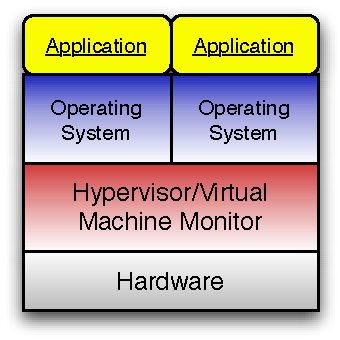
\includegraphics[scale=.75]{architecture-with-virtualization}
  \caption[Virtualization     architecture]{The    so-called    bare-metal
    virtualization: A  virtual machine  monitor runs as  small ``operating
    system''  on  the  real  hardware  and  provides  access  for  virtual
    machines.}
  \label{fig:arch-virt}
\end{figure}

This  kind   of  virtualization  is  called   ``full''  or  ``bare-metal''
virtualization  ---  an operating  system  running  in  a virtual  machine
provided by the  VMM thinks it runs on real  hardware. An abstract picture
of such an architecture is shown in Figure~\ref{fig:arch-virt}.

\section{Virtualization techniques}
\label{sec:techniques}

According   to    the   Church-Turing~Thesis   \cite{church_turing_thesis}
\emph{``Any real-world  computation can  be translated into  an equivalent
  computation involving  a Turing machine.''}, every  computer can simulate
any other computer.

\bigskip

In Figure~\ref{fig:arch-novirt} is  shown, how a non-virtualized environment
may  look like  --- it  consists of  the physical  hardware,  an operating
system running  on that hardware and  some applications running  on top of
the operating system.

\begin{figure}[htbp]
  \centering
  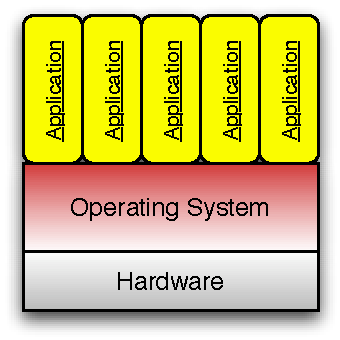
\includegraphics[scale=.75]{architecture-without-virtualization}
  \caption[Architecture  without virtualization]{A  computer  system, that
    does not make use of virtual machines.}
  \label{fig:arch-novirt}
\end{figure}

The  following  sections  describe  some  techniques,  how  this  physical
hardware may be split up, so that  two or more virtual machines can run on
top of it without knowing and most important without harming each other.

\subsection{Partitioning}
\label{sec:vt-partitioning}

The first virtualization technique  bases on partitioning of the available
hardware \cite{borden89}.   It is available  since the 1960s and  has been
provided  by  two  approaches  ---  a software  approach  and  a  hardware
approach.

\subsubsection{Software partitioning}
\label{sec:softw-part}

The IBM CP/67  has been the first operating  system which provided virtual
machine support, it  was running on the System/360 Model  67 and was first
available in 1967 \cite{borden89}.

As described earlier, the CP gave each user a virtual machine on which the
CMS (a  single user  operating system) was  running and provided  the user
with command processing and information management functions. Each virtual
machine was ``copy'' of the base hardware architecture, it was possible to
run OS/360 in  a virtual machine and ``in fact, even  CP/67 itself was run
"second  level" in a  virtual machine  for the  purposes of  debugging and
testing \cite{borden89}''.

\subsubsection{Hardware partitioning}
\label{sec:hardw-part}

Hardware partitioning is an enhancement over software partitioning and was
introduced  by  the  IBM   \emph{System/370  158  MP}  and  \emph{168  MP}
systems. In 1967,  IBM introduced multiprocessor versions of  Model 65 and
67, which  provided duplexed hardware to achieve  tolerance against single
hardware failures.  By  splitting up the whole system  into two sides, two
separate systems could be created  which ran totally independent from each
other.

\subsection{Emulation}
\label{sec:emulation}

This kind of virtualization  simulates a complete hardware architecture in
all  details. By  that every  operating system  and  therefore application
which has been  developed for that particular application  may be executed
within the emulator. Some examples are:
\begin{itemize}
\item  \emph{Wine \cite{wine}}  --- Wine  is  not quite  an emulator,  but
  nonetheless I put it in this list, too. It emulates the Windows API, but
  executes many functions directly  on the underlying x86 hardware without
  emulating each instruction.
\item \emph{Bochs  \cite{bochs}} --- this  is a very portable  open source
  IA-32 PC emulator.  Each machine  instruction will be interpreted and is
  handled in software.  This emulator may for instance be  used to run x86
  code on a PowerPC platform.
\item  \emph{QEMU  \cite{qemu}} ---  this  is  both  an emulator  and  an
  virtualizer, since  it support  two modes of  operation. As  an emulator
  each instruction  gets interpreted  as it is  the case  of \emph{bochs},
  \eg it is possible  to emulate an ARM processor on  your PC. To achieve
  better  performances a  technique called  \emph{dynamic  translation} is
  used.   Running as  a virtualizer,  QEMU is  able achieve  nearly native
  performance, since most of the instructions are directly executed on the
  host CPU --- to make this possible a kernel module (QEMU accelerator) is
  required.
\end{itemize}

\subsection{Application virtualization}
\label{sec:appl-level-virt}

The Java virtual machine \cite{java} is a well-known example for this kind
of virtualization. A program written in the Java language is compiled into
a  \emph{Java   byte  code}  and  will   be  executed  by   the  JVM  upon
execution. The virtual machine  and the operating environment together are
called the \emph{Java runtime environment}.

To  improve  execution performance,  an  additional  component called  the
\emph{Java hot-spot compiler} translates small portions of often used code
segments into  machine code (a technique  called ``dynamic translation''),
the translated code can also be cached and therefore be reused later.


\subsection{Operating system-level  virtualization}
\label{sec:oper-syst-level}

This kind  of virtualization  uses the  same kernel for  the host  and all
guest  systems  ---  the  guests  run  ``within''  the  host  environment.
Examples include Solaris Containers and FreeBSD jails.

FreeBSD jails are  used to shut a service or  a special server application
in  its own  environment  --- therefore  prohibiting  an application  from
\emph{leaving}   (\ie accessing  data   outside   its  environment)   the
file-system area which an administrator has reserved for it.

\subsection{Para-virtualization}
\label{sec:paravirtualization}

Typically, the  instructions (or  most of them)  of a virtual  machine are
directly  executed  on  the  underlying  physical processor  to  get  best
performance  results.  Unfortunately, some  instructions are  simply ``not
designed'' to be virtualized at all (see \ref{sec:x86-problems}) --- those
instructions  perform changes  or  query the  state  of some  part of  the
physical hardware, but need not to be run in ``privileged mode''.

All instructions that  cannot be virtualized have to  be rewritten by the
VMM before  they get executed, that  means a loss  in performance.  VMWare
\cite{vmware} for instance runs as  a stand-alone application on top of an
operating system  (supported by  some extensions to  the kernel)  and uses
this kind of  binary rewriting, see Figure~\ref{fig:arch-userspace-virt} for
a schematic overview.

\begin{figure}[htbp]
  \centering
  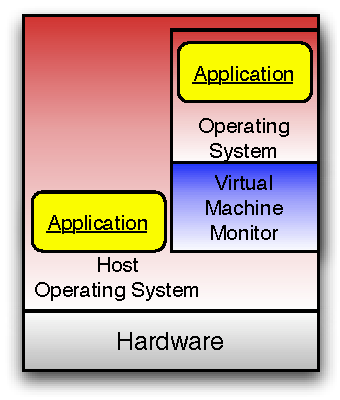
\includegraphics[scale=.75]{architecture-userspace-virtualization}
  \caption[Virtualization  in  the   user-space]{Example  for  the  VMWare
    virtualization software, which  runs as an application on  top of some
    operating system}
  \label{fig:arch-userspace-virt}
\end{figure}

The Xen  hypervisor \cite{xen} however,  avoids this problem  by providing
its  own ``architecture''  to which  a guest  operating system  has  to be
ported --- they call an operating  system which has been ported to the Xen
architecture  ``Xen-aware''.   The  proposed  architecture  contains  only
``small''  modifications  to  the  real hardware  architecture,  \ie they
mainly modify the non virtualizable instructions.

The term \emph{para-virtualization} has first been used in the description
of  \emph{Denali}  \cite{denali}  (see Figure~\ref{fig:arch-para-virt}).  In
this  case the  VMM presents  its virtual  machines with  a \textbf{nearly
  identical} copy of the underlying hardware, but the virtualized hardware
is much less complex than the physical hardware (no BIOS, simpler devices,
etc.).  The  modifications to  the virtual hardware  architecture require,
that the operating system running a virtual machine must be aware of those
modifications --- legacy  systems cannot be executed as  long as they are
not ported to the new architecture.

\begin{figure}[htbp]
  \centering
  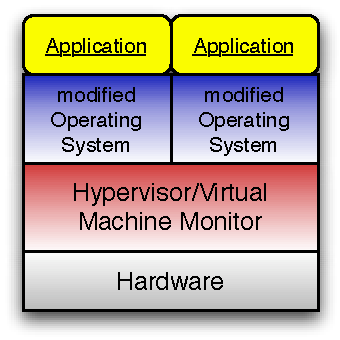
\includegraphics[scale=.75]{architecture-with-paravirtualization}
  \caption[Para-virtualization architecture]{An architecture that uses the
    para-virtualization technique}
  \label{fig:arch-para-virt}
\end{figure}

\subsection{Problems with the x86 architecture}
\label{sec:x86-problems}

In \cite{schroeder72} a hardware implementation of \emph{protection rings}
mainly  used  for  the  MULTICS  operating system  are  described.   These
\emph{protection rings} are still present in todays processors and so they
are in the x86 architecture.

Protection  rings are  used to  separate ``privileged''  instructions from
``unprivileged''  ones. The  x86  architecture provides  a  total of  four
rings, with ring 0 being the most privileged one --- typically only two of
them are used: ring 0 is  occupied by the operating system kernel and ring
3  is used  to executed  user  programs.  Popek  \cite{popek74} assumes  a
processor architecture,  that provides two modes  of operation, supervisor
and  user  --- so  the  requirements  which have  to  be  fulfilled by  an
architecture to be virtualizable apply to the x86 architecture as well.

Popek identifies three kinds of instructions --- privileged, sensitive and
innocuous \cite{popek74}:

\begin{itemize}
\item \emph{Privileged}  instructions are those, that must  be executed in
  supervisor mode and trap if  executed in user mode. The x86 architecture
  has many  of these instructions, but  all of them  raise a \emph{general
    protection fault} if executed in user mode \cite{robin00analysis}.
  
\item \emph{Sensitive} instructions are those, that ``have a major bearing
  on     the     virtualizability     of    a     particular     machine''
  \cite{popek74}.  Generously  speaking,  they  change the  state  of  the
  hardware in some way without trapping.
  
\item \emph{Innocuous} instructions are all those which do not do any harm
  to the state of the processor from the VMM point of view.
\end{itemize}

Virtualization on the x86 architecture is typically implemented by running
the VMM in privileged mode and the virtual machines in user mode. For this
to  be successful,  all ``sensitive''  instructions \cite{popek74,popek75}
must trap into the VMM, so that they can be correctly emulated.

It  has been  analyzed that  all  privileged instructions  of the  Pentium
instruction  set correctly  trap (\ie they  raise a  ``general protection
fault'')   and  can   be  handled   by  the   VMM  \cite{robin00analysis}.
Unfortunately    there    are    seventeen    instructions    which    are
\textbf{sensitive}  and  \textbf{unprivileged},  so  they  do  \textbf{not
  trap}.

I think  that is  the main  reason, why full  virtualization has  not been
implemented for the x86 architecture for a long time.

Intel  and AMD,  the leading  manufactures for  x86 based  processors, are
currently  developing   hardware  support  for   virtualization,  so  that
unmodified guest operating systems can be run under a VMM.

\section{The Xen hypervisor}
\label{sec:xen-hypervisor}

\begin{quote}
  ``The term “hypervisor” is applied to computer systems that present a very
basic user  program interface ---  one which is  so nearly identical  to a
particular computer machine interface that an operating system intended to
support  such machines  may serve  as  a hypervisor  user program  without
software modification.'' \cite{hendricks79}
\end{quote}

\bigskip

Xen \cite{xen}  is a virtualization  technology to share a  given physical
machine  using smaller  virtual machines  (\gls{glo:VM}s).  Each  of these
\gls{glo:VM}s has their own main memory, file space, access to one or more
virtual  CPUs and everything  else that  is required  to run  an operating
system.  Xen belongs to the  hosted virtualization group, which means that
the \gls{glo:VMM} still  requires an operating system to  run and does not
represent a stand-alone operating system itself.

Older  versions  of  the   Xen  virtual  machine  monitor  only  supported
para-virtualization,   i.~e.~each  guest  operating   system  had   to  be
explicitly ported to the architecture  provided by Xen.  Since version 3.0
the  special  hardware assistance  for  virtualization  provided by  Intel
(Intel-VT) and AMD (AMD-V or Pacifica) is supported.

\begin{figure}[htbp]
  \centering
  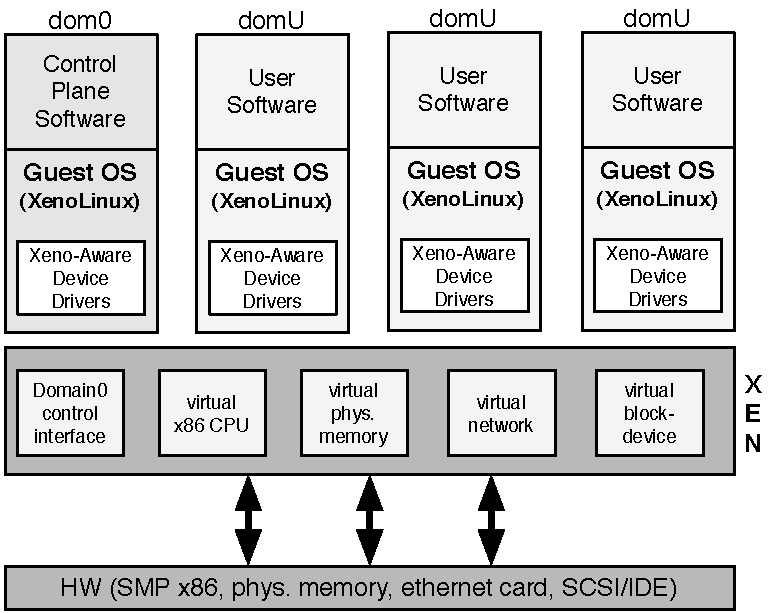
\includegraphics[height=8cm]{xen-architecture}
  \caption[Xen architecture]{The structure of a system running the Xen
    hypervisor and several user domains (taken from \cite{xen-art})}
  \label{fig:xen-architecture}
\end{figure}

Xen  virtual machines  (see Figure~\ref{fig:xen-architecture})  are called
``domains''  and   the  top-level  or   most  privileged  one   is  called
\texttt{Domain-0}  --- or  \texttt{dom0} for  short ---  this is  the one,
which runs the control and management programs that are required to create
new virtual machines.  The  virtual machine instances beside \texttt{dom0}
are called ``user  domains'' --- or \texttt{domU}s for  short --- they are
less privileged and their access to the hardware is controlled and managed
by the hypervisor running in \texttt{dom0}.

The  operating  system  running  within  a user  domain  accesses  virtual
hardware provided by  the Xen-architecture --- SCSI or  IDE controllers to
access virtual hard drives, network interface cards, virtual CPUs, graphic
card and so on.


\section{Benefits of virtualization}
\label{sec:benefits}

To  satisfy customer  demands,  not a  single,  general purpose  operating
system  can be  used, over  the time  dozens of  specialized  systems have
evolved --- for instance on  consumer desktop systems one can find Apple's
MacOS,  Microsoft   Windows,  some  Linux  distribution   with  a  desktop
environment,  on cluster  systems  or  on systems  which  have to  provide
outstanding  security and availability  typically other  operating systems
are  used   (Linux  for  instance,  may   be  an  exception   due  to  its
adaptiveness).  Each  system has been designed  to address the  needs of a
large segment of the marketplace \cite{borden89}.

\bigskip

The following list are reasons, why multiple operating systems may need to
coexist and  even be used in the  same establishment at the  same time and
how virtual machines fit into that \cite{borden89,virtualization-overview}:

\begin{itemize}
\item  \emph{Diverse Workload}  --- in  large establishments  it  is often
  required, that  different computing  requirements must be  fulfilled. An
  airport, for instance, requires  a highly responsive reservation system,
  a  database system  for aircraft  maintenance  and parts  and a  general
  purpose system for payroll and planning.
\item  \emph{Test  and  development}   ---  many  companies  require  high
  availability and stability of  their computing components, but they also
  may want to test, develop  and deploy new software or software versions.
  
  Here at  the Fraunhofer ITWM,  for instance, SuSE  Linux is used  as the
  operating system for many desktop systems. To provide stability, updates
  have to be tested prior deploying them everywhere.

  The same holds for application  development --- a company will have some
  productive system running the developed application, and this system has
  to be available  24 hours a day. Clearly,  development cannot take place
  on  the production  machines, since  the  probability of  a breakage  is
  simply  too  high ---  machines  solely  dedicated  for development  are
  required.
\item \emph{Backup  and recovery} --- server  applications which represent
  important  components   for  the  daily   work  (\eg database  systems,
  web-servers etc.) must  be available all the time. A  nice thing to have
  in such  a situation  is automatic recovery  from failure ---  to reduce
  down-time two systems can be used: one of them is the productive system,
  the  other one  is a  backup system  that is  an exact  ``copy''  of the
  productive system  and just waits  for a failure  of the other.   Upon a
  system failure  in the  productive system, the  backup system  will take
  over.
\item  \emph{Platform  independent development}  ---  over  the time  many
  different  operating  systems have  evolved  ---  various Unix  flavours
  (FreeBSD, Linux for  instance), DOS, Microsoft Windows, Mac  OS, just to
  name some of them --- not all of them are compatible to each other.

  Application developers who  want to develop an application  that runs on
  several of these operating systems are required to port and verify their
  application on each  target system and maybe on  several versions of the
  same target system.

  One way  is to have  an extra machine  with the target  operating system
  installed on  it just for testing  and porting issues ---  that not only
  imposes energy  costs but also maintenance  costs.

  The other way is to use  virtual machines instead of actual machines ---
  each virtual machine runs a version of a target operating system.
\item  \emph{Server consolidation} ---  a common  approach for  many small
  companies is to have one server on which runs for instance a web server,
  some content management system with a database as its back-end under the
  same  operating system.

  That approach  may involve security problems,  since if just  one of the
  services   contains  a   security  hole,   the  whole   system   can  be
  compromised. Using virtual  machines for each of the  services, the only
  system  that is  now compromised  is the  one providing  this particular
  service.
\end{itemize}

\section{Usage scenarios}
\label{sec:usage}

\subsection{Virtual machines in a grid environment}

In  a grid  environment ---  roughly  spoken that  is a  network of  many,
possibly  heterogeneous  resources  ---  the problem  occurs,  whether  an
application can be run on a  specific computing resource or not. There are
several ways to cope with that:

\begin{itemize}
\item All computing  nodes are required to have  all possible applications
  installed --- depending on the problems  which are to be computed in the
  grid, this can be thousands.
\item The  available applications  in a particular  grid are limited  to a
  small maintainable number.
\item  The grid  contains an  information  database which  can be  queried
  whether an application is available on  a given resource or not --- that
  could also mean to query the resource in question on demand.
\item  Only truly  platform independent  applications are  allowed  --- by
  ``truly platform independent'' I mean  that they are not only written in
  a platform independent language, but can also be effectively executed on
  each supported platform.
\end{itemize}

The  proposed Xen-based  execution environment  addresses this  problem by
allowing an user to ``execute'' a complete machine image --- therefore any
user application can be executed.

\subsection{On-demand server deployment}
\label{sec:demand-serv-depl}

Another thing which  could be done with an  execution environment based on
virtual  machines is  ``on-demand server  deployment'', that  is executing
some  sort of  server  application on  a  remote resource  only  if it  is
required.

Assume  a  group  of  people  who  want to  play  a  multi-player  on-line
game. With virtual  machines, it is easily possible for  them to acquire a
well-connected computing resource to  execute the game-server only for the
duration of their on-line play.

Or think of a web-server with some new, but untested extensions, you could
simply deploy  a virtual machine  which contains that web-server  and test
the extensions.

\section{Related work}
\label{ref:related-work}

This  work is surely  not the  only one,  which provides  remote execution
using virtual machines.

\subsection{Amazon EC2}

The \emph{Amazon Elastic Computing Cloud} (EC2, \cite{amazon-ec2}) is part
of the \emph{Amazon  Web Services} project and provides  a web service for
remote execution of user provided virtual machine \gls{glo:image}s.

Amazon provides  you with  a personal storage  area where you  can deposit
arbitrary data  (such as \emph{Amazon Machine Images})  --- another Amazon
web service is used in this case: the \emph{Amazon Simple Storage Service}
(S3).  With the files within your  storage area, you are able to create as
many virtual machines  as you like. Through web service  calls or by using
one  of the  various  command line  tools,  you can  start, terminate  and
monitor you instances.

\subsection{The XenoServer Open Platform}

The  XenoServer Open  Platform is  an implementation  of  the \emph{global
  public   computing}  paradigm   \cite{kotsovinos05}.  It   provides  the
execution of \emph{any code} from \emph{any user} \emph{anywhere}.

Servers \emph{advertise} themselves  and clients \emph{select} the servers
on which their computations or services shall be deployed. After selection
of the servers,  clients send the deployment specification  to each one of
the servers. A server may then  accept or decline the request according to
local policies or resource requirements.


\subsection{How this work is different}

All of the  presented related work provide a user  with the possibility to
execute his application on a  remote virtual machine.  The application may
be untrustworthy and uncooperative. To provide Grid-semantics to the user,
one can install any middleware withing the created virtual machine.

My work differs  in the way how jobs are handled:  I take virtual machines
just as  \emph{containers} for  some job and  provide \emph{execute/return
  result}      semantics      along      with     specialized      staging
operations. Nonetheless, the execution environment which is here proposed,
can also be used to run any Grid-middleware a user demands.


%%% Local Variables: 
%%% TeX-master: "main.tex"
%%% End:
